\documentclass{article}
\usepackage{tabularx}
\usepackage{amsmath}
\usepackage{graphicx}
\usepackage[top = 2cm, bottom = 2cm, right = 2cm, left = 2cm]{geometry}
\usepackage{cite}
\usepackage[final]{hyperref}
\usepackage{listings}
\hypersetup{
	colorlinks=true,
	linkcolor=blue,
	citecolor=blue,
	filecolor=magenta,
	urlcolor=blue         
}

\begin{document}

\title{Practicle 5\\Debugging a CUDA application}
\date{30/01/19}
\maketitle

\begin{abstract}
	
\end{abstract}

\section{Nsight}
Nsight is a development environement for CUDA. This tool is integrated into Visual Studio. When you run you program through Nsight you can reach breakpoint into your kernel. Frist you need to specify your application to generate GPU Debug Information. Go to the Property panel of your project and go on the Device section of CUDA C/C++. Here you can enable the Generate GPU Debug Information (Yes (-G)). Now we can use breakpoint into our kernel. Put one breakpoint after the index computation and run your program. You can read in debug mode the value of your index for the first thread of the first block. Be carefull, adding the -G debug information add check on your kernel and use more registers. Sometime you may reduce the number of thread per block for debugging. 
\subsection{Warp Info}
Most of the time debug only the first thread solve problem because we use SIMD architecture. However, if there is a branch in the kernel you may want to debug another thread. On the Nsight panel, open Windows/Warp Info.

\begin{figure}[h]
	\centering
	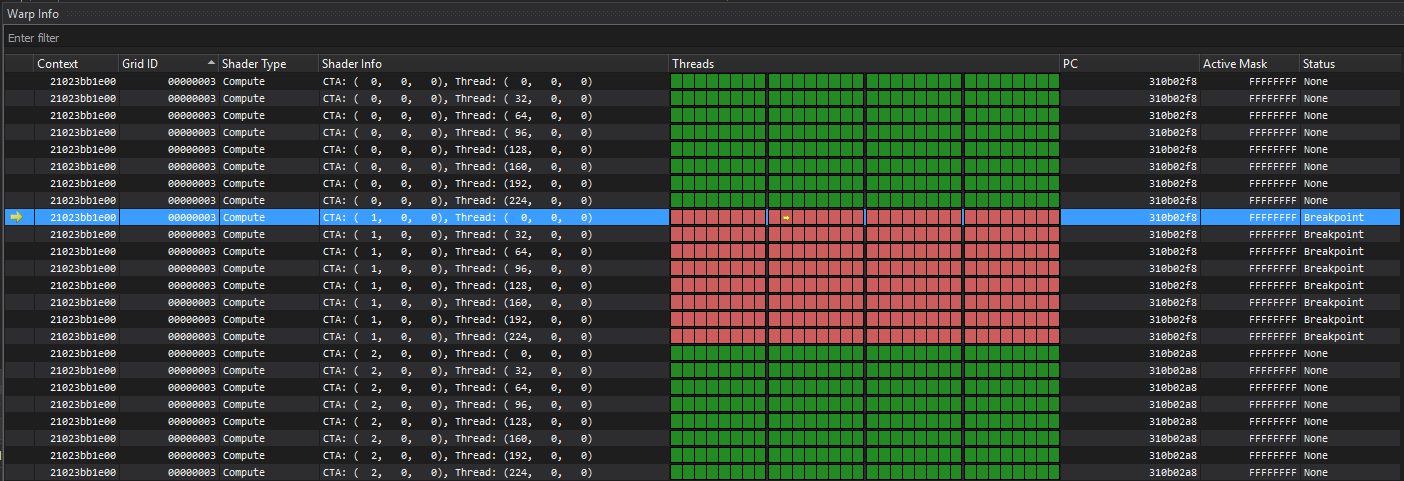
\includegraphics[scale=0.47]{figures/warpinfo.png}
	\caption{Warp Info}
\end{figure}

You can see several color infos for each warps. If it is red is beause the execution reach the breakpoint. If it is green it's mean the thread is active. There is 8 threads states.

\begin{figure}[h]
	\centering
	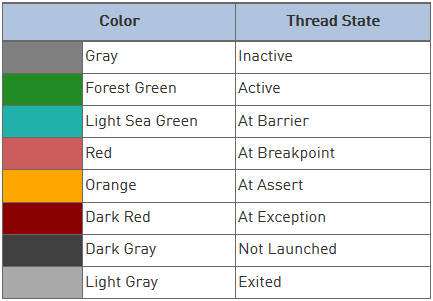
\includegraphics[scale=0.6]{figures/threadstate.png}
	\caption{Warp Info}
\end{figure}

\newpage
\subsection{Lanes}
The lane section allow us to debug threads for the active warp. We can find the same informations as the warp info. If you change the current warp on the warp info it will impact this window too.
\begin{figure}[h]
	\centering
	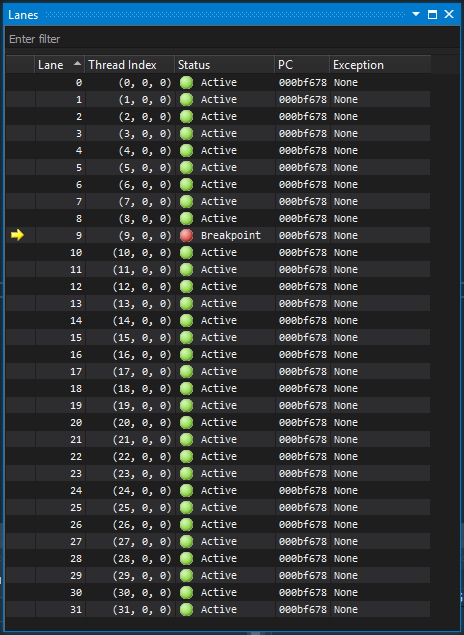
\includegraphics[scale=0.6]{figures/lanes.png}
	\caption{Warp Info}
\end{figure}

\newpage
\subsection{GPU Registers}
Sometime you may need to see the disassembly code for debugging (Right clic on your code/Go to disassembly). You can fallow the value stored into the GPU register on this last window.

\begin{figure}[h]
	\centering
	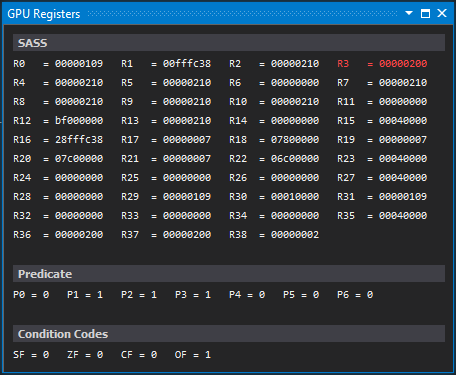
\includegraphics[scale=0.6]{figures/register.png}
	\caption{Warp Info}
\end{figure}

\newpage
\section{Test limits of your program}
\subsection{Reach the maximum of the callstack}
We see on the last practical how to grab an error. Now we'll try to get errors. Create a recursive function called more than 100 times and look at the error throwed. It is because you don't have enought memory for your stack. You can get your device stack size in this way:
\begin{lstlisting}
	size_t value;
	cudaDeviceGetLimit(&value, cudaLimitStackSize);
\end{lstlisting}
And if you want to modify this limite just call:
\begin{lstlisting}
	cudaDeviceSetLimit(cudaLimitStackSize, value);
\end{lstlisting}

\subsection{Branches}
Into on of your simple kernel (like the clear color), add a if statement to do the job only for the half of the threadIdx.
\begin{lstlisting}
	if (threadIdx.x < 16) {
		for (int i = index; i < w*h; i += stride) {
			image[i] = backgroundColor;
		}
	}
\end{lstlisting}
On the Warp Info panel we can see the half of the thread are disabled.

\section{Performance analysis}
On the Nsigh panel you can start the Performance analysis tool. You just need to check the radio button Profile CUDA Application and on the Application Control panel click on Launch. This action will profile each kernel of your application. If needed you can specify which kernel you want to profile.\\
\subsection{Latency and Occupancy}
Latency systems oriented like CPU use speculative fetching, branch prediction and large caches to avoid the delay to get data computed. For SIMT architecture we talk about  occupancy. It is the mesure of thread parallelism. If we look into a thread we are talking about Instruction-level Parallelism. In this exemple a and d can be computed at the same time to avoid latency:
\begin{lstlisting}
	a = b + c
	d = e + f
	g = a + d
\end{lstlisting}
Remenber that more the system use his threads active more the application is efficient.\\
On the result of the performance analysis tool you can see on the CUDA launches all informations relatives to your kernel.\\
Identify heavy kernels and try to split them into smaller process. For exemple we can create a kernel named computeStartRay to compute an image that store data instead of pixel color. We chose an camera origin on (0, 0, 0) so the Red value can store the X value of the ray direction, same for Green and Blue.

\end{document}